\documentclass{article}
\usepackage[spanish]{babel}
\usepackage[utf8]{inputenc}
\usepackage{graphicx}
\usepackage{wrapfig}
\usepackage{amssymb, amsmath}
\setlength{\parindent}{0cm}
\title{Resumen cálculo de cimentaciones}
\author{MakerGarage}
\date{Marzo 2021}



\begin{document}

\maketitle
\begin{center}
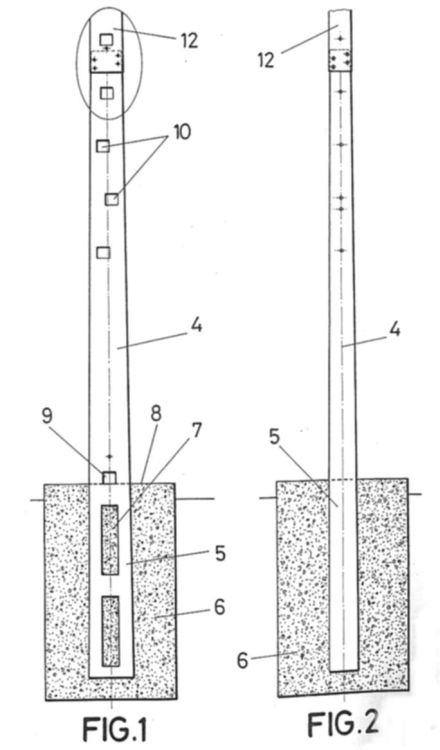
\includegraphics[trim={0 10 cm 0 0},scale = 2,clip]{assets/img/Portada.jpg}
\end{center}
\newpage
\tableofcontents
\newpage

\section{Cimentaciones Mono-bloque}
    \subsection{Introducción}
    La cimentación mono bloque presenta dos momentos, un momento solicitante de vuelco y un momento estabilizador (compuesto por dos momentos). La metodología de resolución que vamos a seguir es el método Sulzberg.
    \begin{center}
    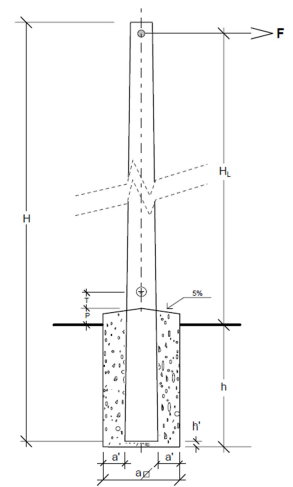
\includegraphics[scale = 1]{assets/img/Cimentacion Monobloque/cimentacion monobloque.png}
    \end{center}
    
    \newpage
    \subsection{Método Sulzberg}
    El método Sulzberg propone que todos los momentos pivotan en el eje de giro situado a $\frac{2}{3}$ de la base (midiendo desde el terreno) y a $\frac{1}{4}$ desde la pared.
    \begin{center}
        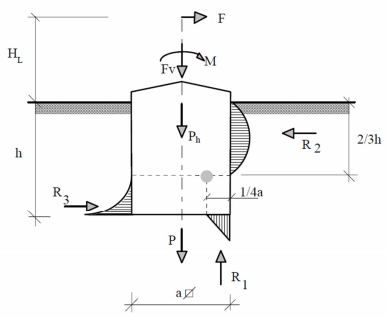
\includegraphics[scale = 1]{assets/img/Cimentacion Monobloque/Momento.png}
    \end{center}
    \\
    Como hemos comentado este método se basa en calcular dos momentos.\\
    
    \begin{array}{cl}
        \bullet & \text{Momento solicitante de vuelco}  \\
        \bullet & \text{Momento restaurador}
    \end{array}\\
    
    El momento solicitante de vuelco es provocado por la tensión del cable F, mientras que el momento restaurador esta compuesto por las reacciones horizontales y las verticales, siendo predominantes las reacciones horizontales.
    \newpage
    \subsubsection{Momento solicitante de vuelco}
    $$
M_{V}=F\left(H_{T}+c-\frac{1}{3} h\right)
$$
\begin{center}
    ó
\end{center}
    $$
M_{V}=F\left(H_{L}+\frac{2}{3} h\right)
$$

En función de los datos que tengamos seleccionamos una u otra.
\\

$\mathrm{F}=$ Esfuerzo nominal del apoyo, más el viento sobre el mismo reducido al punto de aplicación para el cálculo.
\\

$\mathrm{H}_{\mathrm{L}}=$ Altura libre del apoyo desde el punto de aplicación de $\mathrm{F}$ hasta la línea de tierra.
\\

$\mathrm{h}=$ Profundidad de la cimentación, en $\mathrm{m}$.
\\

En apoyos de forma troncopiramidal el esfuerzo del viento se aplica en
$$
H_{0}=\frac{H}{3} \frac{d_{1}+2 d_{2}}{d_{1}+d_{2}}
$$
Siendo $\mathrm{d}_{1}$ y $\mathrm{d}_{2}$ las anchuras o diámetros en el empotramiento y en la cogolla, respectivamente.
\\

En el caso de tener que calcular el momento de vuelco de la peana sobresaliente del terreno:

$$M_{V 2}=F_{V_{\text {poama }}} \cdot\left(\frac{h_{p}}{2}+\frac{2}{3} h\right)=q \cdot S \cdot\left(\frac{h_{p}}{2}+\frac{2}{3} h\right)=q \cdot S \cdot\left(\frac{h_{p}}{2}+\frac{2}{3} h\right)$$
\\
Siendo $q$ 100 (según reglamento).
\\
$S$ es ($a \cdot h_p$).
\newpage
\subsubsection{Momento restaurador}
\textbf{Momento restaurador Horizontal $M_1$}
$$M_{1}=139 \cdot C_{2} \cdot a \cdot h^{4}$$
$C_2$ es la compresibilidad del terreno a 2m
\\

\textbf{Momento restaurador Vertical $M_2$}
$$M_{2}=P \cdot a \cdot\left[0,5-\frac{2}{3} \sqrt{\frac{P}{2 \cdot a^{3} \cdot C_{h} \cdot 10^{6} \cdot \operatorname{tg} \alpha}}\right]$$
\\
Siendo:
\\
$C_{h}=h \cdot \frac{C_{2}}{2}$\\

$P=P_{\text {Apoyo }}+P_{\text {Hormigin }}=P_{\text {Apoyo }}+V_{H} \cdot \delta_{H}$ \\

$V_{H}=a^{2} \cdot\left(h+h_{p}\right)$

\subsubsection{Comprobación de hipótesis}
\\

$$ M_{V} \cdot C S \leq M_{1}+M_{2}$$
\newpage
\section{Cimentaciones de patas separadas}
    \subsection{Introducción}
        En las cimentaciones de patas separadas se presentan dos esfuerzos causados por la tensión del cable, un esfuerzo de arranque y otro de compresión tal y como observamos en la figura siguiente.
        \begin{center}
            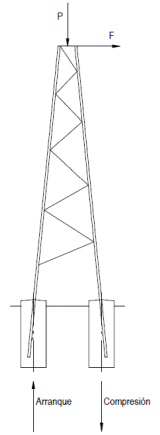
\includegraphics[scale=1.3]{assets/img/Patas Separadas/Cimentacion de patas separadas.png}
        \end{center}
        
    \newpage
    \subsection{Tipos de cimentaciones de patas separadas}
        Dentro de las cimentaciones de patas separadas podemos distinguir principalmente dos tipos:
        \begin{itemize}
            \item Sección cuadrada \begin{center}
            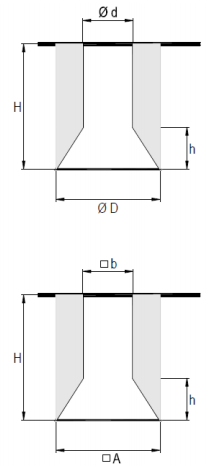
\includegraphics[trim={0 0 0 6.5cm},clip]{assets/img/Patas Separadas/Seccion circular o cuadrada.png}
            \end{center}
            \item Sección circular \begin{center}
            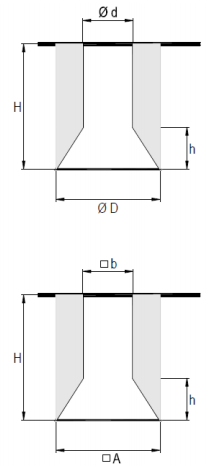
\includegraphics[trim={0 6.5cm 0 0},clip]{assets/img/Patas Separadas/Seccion circular o cuadrada.png}
            \end{center}
        \end{itemize}
        Apreciamos la diferencia en la anotación de cota lineal o de diámetro. Por otro lado cabe destacar que la cimentación comienza a ensancharse en su base inferior a partir de h,a este engrosamiento se le conoce como \textbf{\underline{pata de elefante}}, y es opcional su utilización o no como veremos a continuación.
    
    \newpage
    \subsection{Hipótesis a calcular}
        Para resolver este tipo de cimentaciones es necesario resolver 3 hipótesis.
        \begin{itemize}
            \item Hipótesis al arranque.\\
                En esta hipótesis verificamos que la cimentación sometida al esfuerzo de arranque soporta dicho esfuerzo.
            \item Hipótesis a compresión \\
                En esta hipótesis verificamos que el terreno soporta el esfuerzo de compresión.
            \item Hipótesis de adherencia \\
                En esta hipótesis verificamos que no hay movilidad entre la pata del apoyo y el hormigón vertido
        \end{itemize}

        Los pasos a seguir para resolver estos ejercicios son los siguientes:
        
        \begin{itemize}
            \item Comprobar hipótesis al arranque
            \begin{itemize}
                \left.
                 \begin{array}{cl}
                 \bullet & \text{Arrancan} \rightarrow  $T_{arranque}$ \\
                \bullet & \text{Comprimen} \rightarrow $ P = P_h + P_t + (P_\beta -\delta{ter} \cdot V_{int})$
            \end{array}
            \right\}
            \rightarrow
            $$P > CS \cdot T_{arranque}$$
            \end{itemize}
            
            \item Comprobar hipótesis a compresión \rightarrow $ \sigma_{t}$
            \item Comprobar hipótesis de adherencia
            
            \left.
            \begin{array}{cl}
                 \bullet & $\theta$ \\
                 \bullet & $F_2$ \\
                 \bullet & $F_{adh}$ \\
                 \bullet & $F_c$ 
            \end{array}
            \right\}
            \rightarrow
            \begin{array}{cl}
                $F_{adh} > 0.75 F_2$\\
            $F_c > 0.75 F_2$
            \end{array}
            
            
        \end{itemize}
        \subsubsection{Hipótesis al arranque}
            {
            \begin{wrapfigure}{r}{0.005 cm}\scalebox{0.75}{
            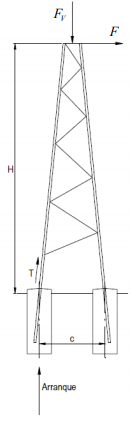
\includegraphics[trim={0 0.5cm 0 0.6cm}]{assets/img/Patas Separadas/Esfuerzo Arranque.png}}
            \end{wrapfigure}
            En esta hipótesis debemos calcular los esfuerzos que intentan arrancar nuestra cimentación por un lado, por otro lado vamos a calcular los esfuerzos que se oponen a dicho arranque y finalmente verificaremos si cumple o no el criterio.\\
            
            \textbf{\underline{Esfuerzos de arranque}}
            \begin{equation*}
                T_{arranque} = \frac{F \cdot H}{2 \cdot c} - \frac{F_v + P_{apoyo}}{4}
            \end{equation*}
            Es importante destacar que el peso del apoyo $P_{apoyo}$ se suele dar en dos partes, el peso del fuste por un lado y el del armado por otro.
            Estos pesos suelen venir en Kg por tanto debemos de sumar ambos pesos y multiplicar por 0'981.
            \\
            
            $F_v$ es el peso del conductor por el número de conductores en daN.
            }
            \newpage
            \textbf{\underline{Esfuerzos de compresión}} \\
            
            Disponemos de 3 esfuerzos que evitan el arranque de nuestra cimentación.
            \\
            
            Recordar que $\delta_{x}$ suele venir en Kg por tanto debemos de multiplicar por 0'981.
            
            \begin{center}
            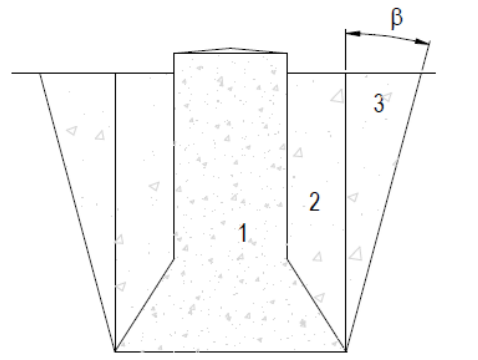
\includegraphics[scale = 0.4]{assets/img/Patas Separadas/Esfuerzo a compresion.png}
            \end{center}
            
            
            \begin{itemize}
                \item\textbf{ Peso del macizo de hormigón.} (1)
                    \begin{itemize}
                        \item Cimentación redonda
                        \begin{equation*}
                        P_h = \delta_{hormigon} \cdot \pi \cdot\left[(H-h)\cdot\left(\frac{d}{2}\right)^2 + \frac{h}{3}\cdot\left(\frac{D^2+D\cdot d + d^2}{4}\right)\right]
                        \end{equation*}
                        \begin{center}
                            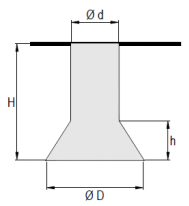
\includegraphics[scale = 0.5]{assets/img/Patas Separadas/cimentacion circular.png}
                        \end{center}
                        \item Cimentación cuadrada
                         \begin{equation*}
                        P_h = \delta_{hormigon} \cdot\left[(H-h)\cdot b^2 + \frac{h}{3} \cdot \left(A^2 +A\cdot b + b^2\right)\right]
                        \end{equation*}
                        \begin{center}
                            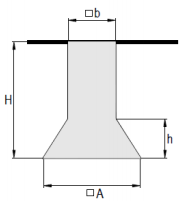
\includegraphics[scale = 0.5]{assets/img/Patas Separadas/cimentacion cuadrada.png}
                        \end{center}
                    \end{itemize}
                    
                \newpage
                \item\textbf{ Peso de las tierras que gravitan sobre el hormigón.} (2)
                
                Este peso ocurre si disponemos de pata de elefante, en caso contrario su valor es 0.
                
                \begin{itemize}
                        \item Cimentación redonda
                        \begin{equation*}
                        P_t = \delta_{terreno} \cdot \left(\pi\cdot H \cdot \frac{D^2}{4} - \frac{P_h}{\delta_h} \right)
                        \end{equation*}
                        \begin{center}
                            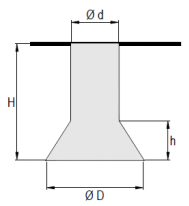
\includegraphics[scale = 0.5]{assets/img/Patas Separadas/cimentacion circular.png}
                        \end{center}
                        \item Cimentación cuadrada
                         \begin{equation*}
                        P_t = \delta_{terreno} \cdot \left(H \cdot A^2 - \frac{P_h}{\delta_h} \right)
                        \end{equation*}
                        \begin{center}
                            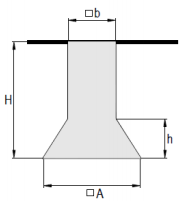
\includegraphics[scale = 0.5]{assets/img/Patas Separadas/cimentacion cuadrada.png}
                        \end{center}
                    \end{itemize}
                
                \newpage
                \item\textbf{ Peso de las tierras según el ángulo natural del terreno.} (3)
                \begin{itemize}
                        \item Cimentación redonda
                        \begin{equation*}
                        \mathrm{P}_{\beta}= \delta_{\text {terr }}\left[\pi \cdot \frac{\mathrm{H}}{3} \cdot\left[\left(\frac{\mathrm{D}}{2}+\mathrm{H} \cdot \tan (\beta)\right)^{2}+\frac{\mathrm{D}}{2} \cdot\left(\frac{\mathrm{D}}{2}+\mathrm{H} \cdot \tan (\beta)\right)+\left(\frac{\mathrm{D}}{2}\right)^{2}\right]-\pi \cdot \mathrm{H} \cdot \frac{\mathrm{D}^{2}}{4}\right]
                        \end{equation*}
                        \begin{center}
                            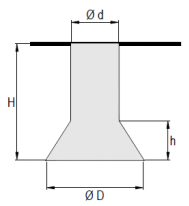
\includegraphics[scale = 0.5]{assets/img/Patas Separadas/cimentacion circular.png}
                        \end{center}
                        \item Cimentación cuadrada
                         \begin{equation*}
                            P_\beta= \delta_{\text {terr }}\left[\frac{H}{3} \cdot\left[(A+2H \cdot \tan (\beta))^{2}+A \cdot(A+2 H \cdot \tan (\beta))+A^{2}\right]-H \cdot A^{2}\right]
                        \end{equation*}
                        \begin{center}
                            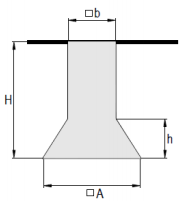
\includegraphics[scale = 0.5]{assets/img/Patas Separadas/cimentacion cuadrada.png}
                        \end{center}
                    \end{itemize}
                Si la separación entre patas es pequeña puede darse el caso de que se produzca \textbf{\underline{interferencia entre cimentaciones}} causando que al peso $P_\beta$ haya que restarle el peso de la tierra de interferencia la cual ha sido eliminada, lo cual se puede observar de manera muy clara en la siguiente imagen.
                \begin{center}
                     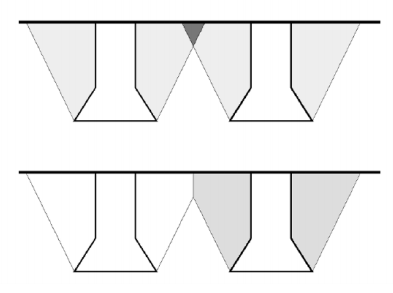
\includegraphics[scale = 0.5]{assets/img/Patas Separadas/interferencia entre cimentaciones.png}
                \end{center}
                Lo que perseguimos es calcular el volumen de terreno que se interfiere para poder calcular su peso como 
                \begin{equation*}
                \delta_{\text {terreno}} \cdot V_{\text {int }}
                \end{equation*}
                \\
                
                \underline{\textbf{Para calcular $V_{int}$ la calculadora debe estar en radianes}}.
                \begin{itemize}
                        \item Cimentación redonda
                         \\
                         La interferencia en cimentaciones se produce si el valor $\mathrm{R}>\mathrm{c} / 2$.
                        $$
                        V_{\text {int }}=\frac{H_{t}}{3}\left[ \cdot R^{2} \cdot \arccos{ \left(\frac{c}{2 \cdot R}\right)}+\frac{c^{3}}{8 \cdot R} \ln \left[2 \frac{\sqrt{R^{2}-\left(\frac{c}{2}\right)^{2}}+R}{c}\right]-c \cdot \sqrt{R^{2}-\left(\frac{c}{2}\right)^{2}}\right]
                        $$
                        Siendo ``c" la distancia entre patas y
                        $$
                        \mathrm{R}=\frac{\mathrm{D}}{2}+\mathrm{H} \cdot \tan (\beta) \quad \mathrm{H}_{\mathrm{t}}=\frac{\mathrm{R}}{\tan \beta}
                        $$
                        \begin{center}
                            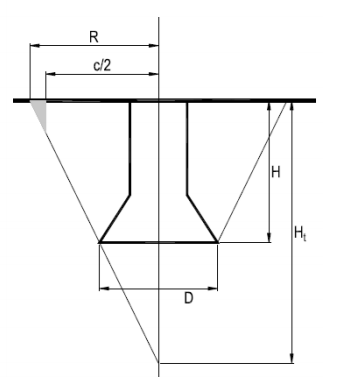
\includegraphics[scale = 0.4]{assets/img/Patas Separadas/interferencia redonda.png}
                        \end{center}
                        \item Cimentación cuadrada
                        \\
                         Para cimentaciones rectas la interferencia se produce si $\mathrm{B}>\mathrm{c} / 2$ y el cálculo es:
$$
V_{\text {int }}=\left(B-\frac{c}{2}\right) \cdot \frac{B-\frac{c}{2}}{2 \cdot \tan (\beta)} \cdot 2 \cdot B
$$
Simplificando:
$$
V_{\text {int }}=\frac{B \cdot(c-2 \cdot B)^{2}}{4 \cdot \tan (\beta)}
$$
Siendo:
$$
\mathrm{B}=\frac{\mathrm{A}}{2}+\mathrm{H} \cdot \tan (\beta)
$$
                        \begin{center}
                            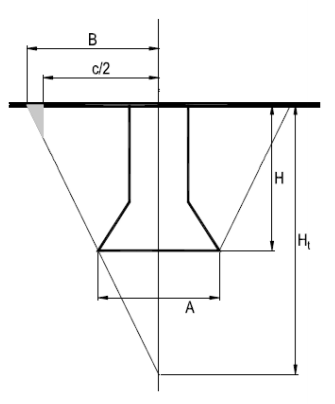
\includegraphics[scale = 0.4]{assets/img/Patas Separadas/interferencia cuadrada.png}
                        \end{center}
                    \end{itemize}
            \end{itemize}
            
        \textbf{\underline{Comprobación de la hipótesis de arranque}} \\
            
            Una vez tenemos calculados tantos los esfuerzos que tracción como los de compresión procedemos a sumarlos obteniendo una $P$ resultante.
            
            $$
            P=P_{h}+P_{t}+\left(P_{\beta}-\delta_{\text {terr }} \cdot V_{\text {int }}\right)
            $$
            Para el correcto dimensionamiento de la cimentación
            $$
            P>C S \cdot T_{a r r}
            $$
            \begin{itemize}
                \item C.S. 1,5 Hipótesis normales
                \item C.S. 1,2 Hipótesis anormales
            \end{itemize}
            
            \newpage
            \subsubsection{Hipótesis a compresión}
            {
            \begin{wrapfigure}{r}{0.005 cm}\scalebox{1}{
            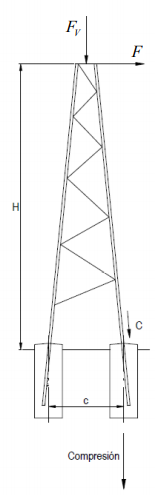
\includegraphics[trim={0 0.5cm 0 0.6cm}]{assets/img/Patas Separadas/Esfuero 2.png}}
            \end{wrapfigure}
            En esta hipótesis debemos calcular los esfuerzos que intentan hundir nuestra cimentación, y debemos de asegurarnos de que el terreno resiste esta presión.\\
            
            El esfuerzo de compresión sobre el montante es:
            $$
            T_{C}=\frac{F \cdot H}{2 \cdot c}+\frac{F_{V}+P_{a p o y o}}{4}
            $$
            Es importante destacar que el peso del apoyo $P_{apoyo}$ se suele dar en dos partes, el peso del fuste por un lado y el del armado por otro.
            Estos pesos suelen venir en Kg por tanto debemos de sumar ambos pesos y multiplicar por 0'981.
            \\
            
            $F_v$ es el peso del conductor por el número de conductores en daN.
            
            \begin{itemize}
                        \item Cimentación redonda
                        \begin{equation*}
              \sigma_{t}=\frac{\frac{F \cdot H}{2 \cdot c}+\frac{F_{V}+P_{\text {apoyo }}}{4}+P_{h}+P_{t}}{\pi \cdot \frac{D^{2}}{4}}
            \end{equation*}
            
            
            \begin{equation*}
                \sigma_{t}=\frac{2 \cdot F \cdot H+F_{V} \cdot c+P_{a p o y o} \cdot c+4 \cdot P_{h} \cdot c+4 \cdot P_{t} \cdot c}{\pi \cdot D^{2} \cdot c}
            \end{equation*}
                        \item Cimentación cuadrada
                         \begin{equation*}
                             \sigma_{t}=\frac{\frac{F \cdot H}{2 \cdot c}+\frac{F_{V}+P_{a p o y o}}{4}+P_{h}+P_{t}}{A^{2}}
                         \end{equation*}
                         
                         \begin{equation*}
                             \sigma_{t}=\frac{2 \cdot F \cdot H+F_{V} \cdot c+P_{\text {apoyo }} \cdot c+4 \cdot P_{h} \cdot c+4 \cdot P_{t} \cdot c}{4 \cdot A^{2} \cdot c}
                         \end{equation*}
                    \end{itemize}
            } 
            Es importante recordar que $A^2$ ó $D^2$ va en cm.
            \\
            
            Una vez tenemos calculada nuestra $\sigma_t$ debemos vereficar que el terreno soporta esta presión.
            $$
            \sigma_{\mathrm{adm}}>\sigma_{\mathrm{t}}
            $$
            \newpage
            \subsubsection{Hipótesis de adherencia}
            En esta hipótesis suponemos que la mitad del esfuerzo lo absorbe el rozamiento entre cimentación y montante y la otra mitad es soportado por los tornillos que están sometidos a un esfuerzo de cortadura.
            \\
            
            \textbf{\underline{Comprobación de la adherencia del montante con el hormigón}} 
            \\
            
            La adherencia acero del montante con el hormigón de la cimentación se puede calcular como:
            $$
            \mathrm{F}_{\mathrm{adh}}=\tau_{\mathrm{adh}} \cdot \mathrm{Sup}
            $$
            La tensión de adherencia se puede calcular como:
            $$
            \tau_{\mathrm{adh}}=0.253 \cdot \sqrt{\mathrm{f}_{\mathrm{ck}}}
            $$
            Siendo $\mathrm{f}_{c k}$ la resistencia característica del hormigón en MPa:
            $$
            \begin{array}{c}
            \mathrm{f}_{\mathrm{ck}}=25 \mathrm{MPa} \\
            \tau_{\mathrm{adh}}=1.265 \cdot 10^5 \mathrm{dPa}
            \end{array}
            $$
            \\
            
            - La superficie de contacto se puede calcular como el perímetro del perfil por la longitud embebida en el hormigón.

El perímetro del perfil en caso de los angulares puede calcularse como 4 veces el lado.
- Dada una tracción máxima a soportar y un perfil dado, la incógnita será la profundidad mínima para soportar esa tracción
- Recopilando términos:
$$
\begin{array}{c}
\quad \mathrm{F}_{\mathrm{adh}}=\tau_{\mathrm{adh}} \cdot \text { Sup } \\
\mathrm{F}_{\mathrm{adh}}=\tau_{\mathrm{adh}} \cdot\left(\mathrm{L}_{\text {anclaje }} \cdot \text { Perimetro }\right) \\
\mathrm{F}_{\mathrm{adh}}=\tau_{\mathrm{adh}} \cdot\left(\mathrm{L}_{\text {anclaje }} \cdot 4 \cdot \text { Lado }\right) \\
\mathrm{L}_{\text {anclaje }}=\frac{\mathrm{F}_{\mathrm{adh}}}{\tau_{\mathrm{adh}}{\cdot 4} \cdot \text {Lado }}
\end{array}
$$
Las longitudes del perfil 200.16 deben ir en metros, es decir 0'2.
\\

- Si los datos son el tipo de angular y la profundidad del anclaje se puede calcular:
$$
\mathrm{F}_{\mathrm{adh}}=\tau_{\mathrm{adh}} \cdot\left(\mathrm{L}_{\text {anclaje }} \cdot 4 \cdot \text { Lado }\right)
$$
\\

La $L_{anclaje}$ viene determinada por el perfil, si nos dicen que es un 200.16 tenemos que poner 0.2

El $Lado$ viene expresado directamente 3.5m normalmente.

            \newpage
            \textbf{\underline{Comprobación de los tornillos a esfuerzo cortante}} 
            \\
            
La cortadura de los tornillos se calcula según la siguiente expresión:
Donde:
$$
\mathrm{F}_{\mathrm{C}}=\mathrm{n} \cdot \frac{0.5 \cdot \sigma_{\text {rotura }} \cdot \mathrm{Secc}}{\gamma_{\mathrm{M} 2}}
$$
\begin{itemize}
    \item n es en número de tornillos
\item$\sigma_{\mathrm{rot}}$ la carga de rotura del material, si nos la dan en Mpa tenemos que multiplicar por $10^5$
\item Secc la sección del tornillo, nos dicen que es un M24 por tanto la sección es $\frac{\pi*0.024^2}{4}$
\item$\gamma_{\mathrm{M} 2}$ Coeficiente parcial de seguridad 1,25
\end{itemize}

\textbf{\underline{Comprobaciones}} 
            \\

            Si $F_{1}$ es el esfuerzo a tracción $y F_{2}$ es el esfuerzo a compresión que se producen sobre los angulares montantes de cada una de las patas y $\theta$ es el ángulo que forma el montante con la vertical, tenemos:
$$
\begin{array}{c}
F_{1}=\frac{F_{t} \cdot H_{t}}{2 \cdot c \cdot(\cos \theta)^{2}}-\frac{F_{V T}}{4 \cdot(\cos \theta)^{2}} \\
F_{2}=\frac{F_{t} \cdot H_{t}}{2 \cdot c \cdot(\cos \theta)^{2}}+\frac{F_{V T}}{4 \cdot(\cos \theta)^{2}} \\
F_{a d h} \geq 0,75 \cdot F_{2} \quad F_{c} \geq 0,75 \cdot F_{2}\\
F_{V T}=F_{V}+P_{\text {apoyo }}
\end{array} 
$$
\\

La longitud mínima de angular embebida en el hormigón debe de ser:
$$
L_{\text {anclaje }} \geq \frac{0,75 \cdot F_{2}}{\tau_{a d h} \cdot 4 \cdot \text { Lado }}
$$

El ángulo puede calcularse como:
$$
\theta=\arctan \left(\frac{\frac{c-a_{cabeza}}{2}}{H_{\mathrm{Libre}}}\right)
$$
\end{document}
